\subsection{Validation}
\frame{\tableofcontents[currentsubsection]}

\begin{frame}{Main Task: Point-wise Valid Upper Bound on Type I Error}
\begin{figure}
    \centering
    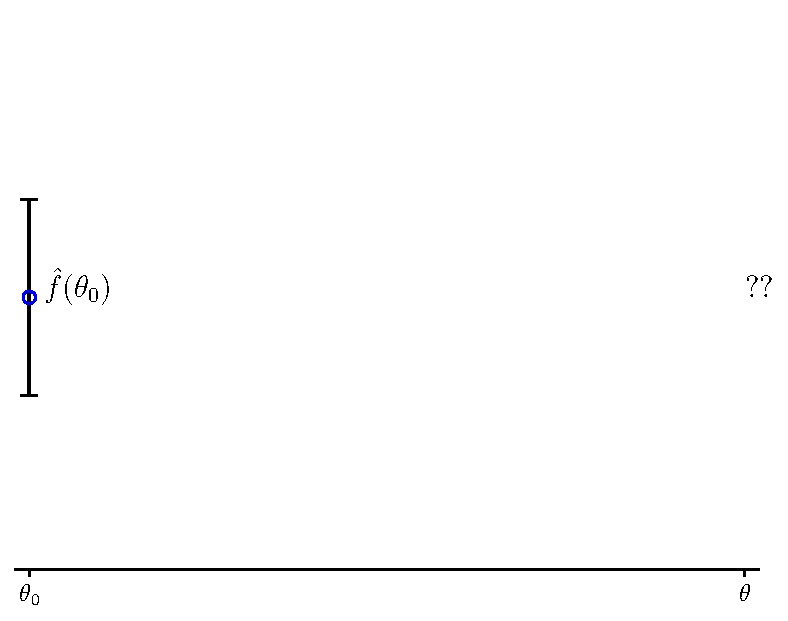
\includegraphics[width=0.75\linewidth]{figs/validation_problem.pdf}
\end{figure}
\begin{itemize}
    \item $X \sim P_\theta$ (known distribution), null space $\Theta$.
    \item Any arbitrary design $\design$.
    \item Clopper-Pearson bound using Monte Carlo estimate $\hat{f}(\theta_0)$.
\end{itemize} 
\end{frame}

\begin{frame}{Claim: Valid Upper Bound on the Type I Error}
\begin{figure}
    \centering
    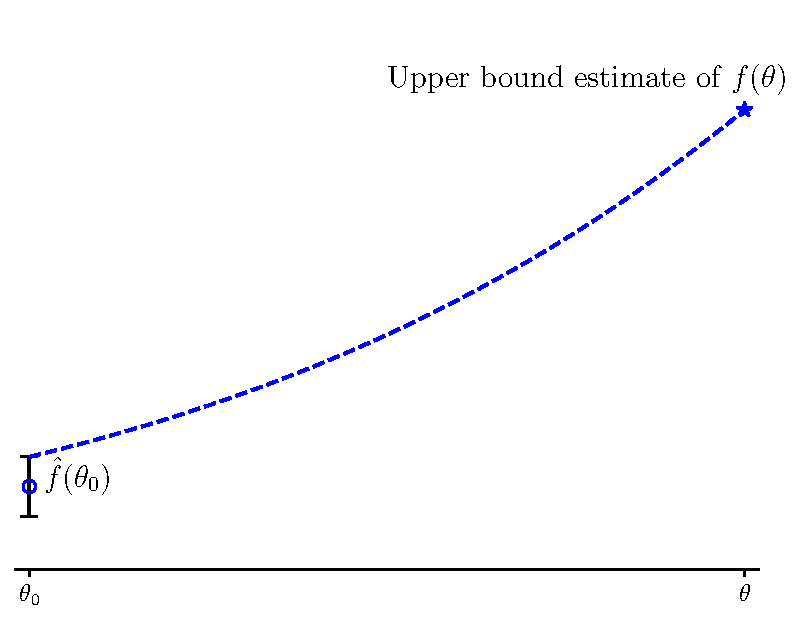
\includegraphics[width=0.95\linewidth]{figs/validation_solution.pdf}
\end{figure} 
\end{frame}

\begin{frame}{Use Tilt-Bound on Upper Bound Estimate!}
\textbf{Monotone Property:}
\begin{itemize}
    \item $a \mapsto U(\theta_0, v, q, a)$ is \textbf{non-decreasing}.
\end{itemize}

\textbf{Validation Proof:} 
\begin{itemize}
    \item $\hat{\eta}$ be a $1-\delta$ upper bound of $f(\theta_0)$.
    \item $\hat{u} := U(\theta_0, v, q, \hat{\eta})$ for any $q \geq 1$.
\end{itemize}
Recall,
\begin{align*}
    f(\theta_0 + v)
    \leq
    U(\theta_0, v, q, f(\theta_0))
\end{align*}
Then,
\begin{align*}
    \prob\pr{f(\theta_0+v) \leq \hat{u}}
    \geq
    \prob\pr{f(\theta_0) \leq \hat{\eta}}
    \geq
    1-\delta
\end{align*}
\end{frame}

\begin{frame}{Use Tilt-Bound on a Grid for the Z-Test}
\begin{figure}
    \centering
    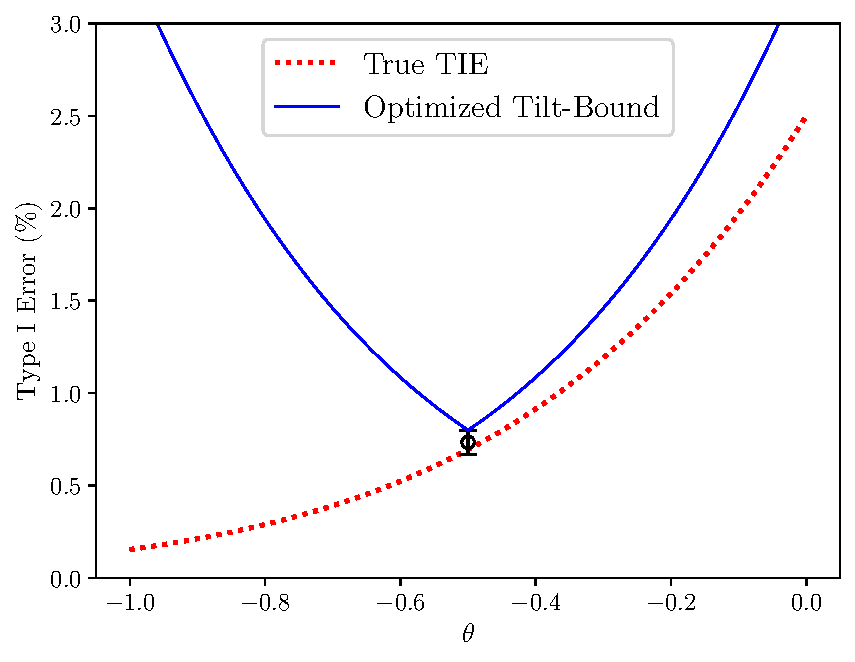
\includegraphics[width=0.95\linewidth]{figs/validation_1.pdf}
\end{figure} 
\end{frame}

\begin{frame}{Use Tilt-Bound on a Grid for the Z-Test}
\begin{figure}
    \centering
    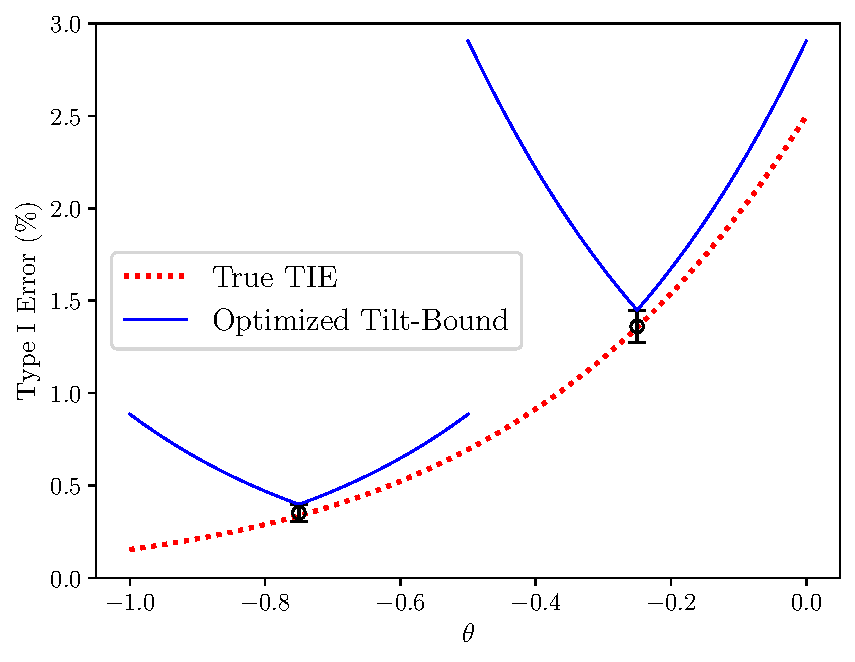
\includegraphics[width=0.95\linewidth]{figs/validation_2.pdf}
\end{figure} 
\end{frame}

\begin{frame}{Use Tilt-Bound on a Grid for the Z-Test}
\begin{figure}
    \centering
    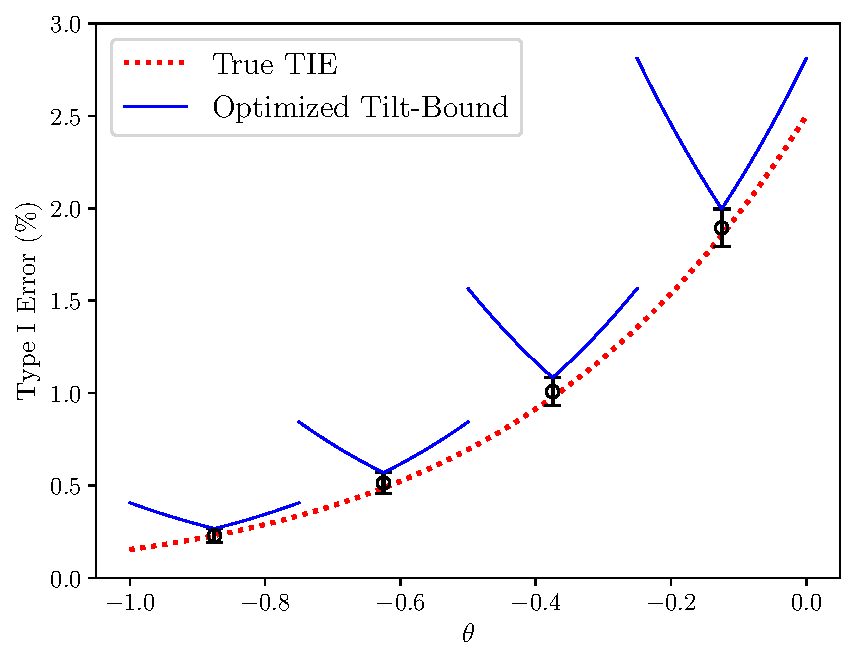
\includegraphics[width=0.95\linewidth]{figs/validation_4.pdf}
\end{figure} 
\end{frame}

\begin{frame}{Use Tilt-Bound on a Grid for the Z-Test}
\begin{figure}
    \centering
    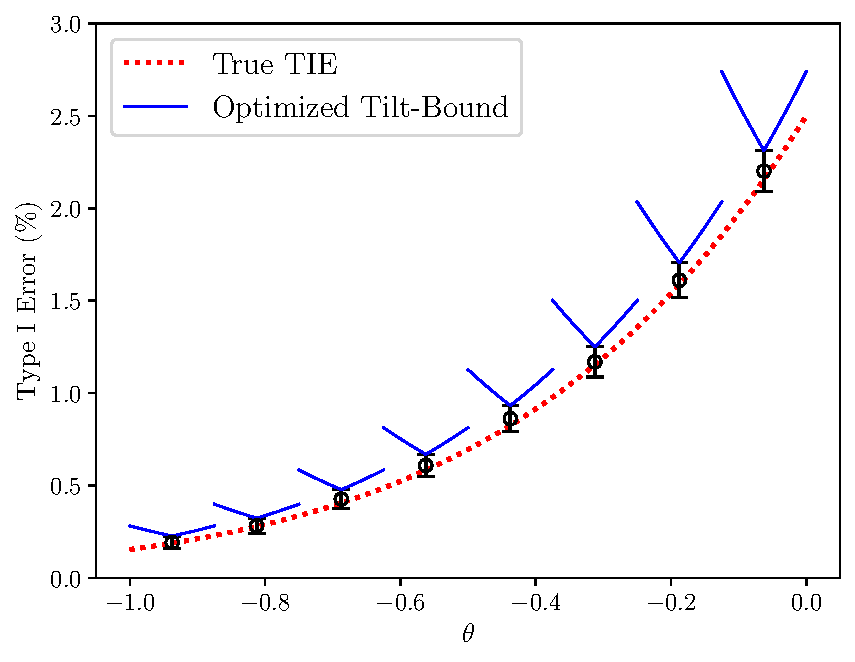
\includegraphics[width=0.95\linewidth]{figs/validation_8.pdf}
\end{figure} 
\end{frame}

\begin{frame}{Use Tilt-Bound on a Grid for the Z-Test}
\begin{figure}
    \centering
    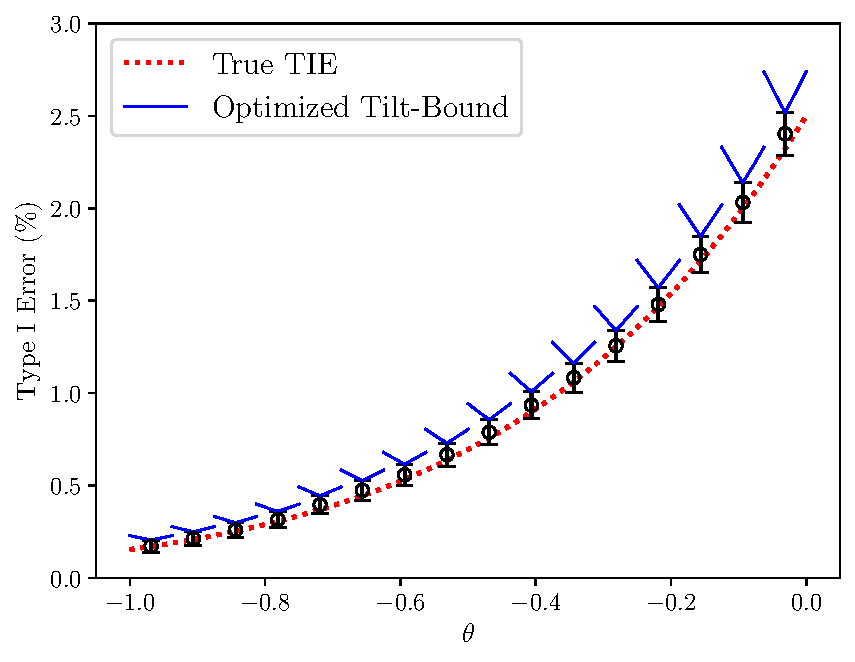
\includegraphics[width=0.95\linewidth]{figs/validation_16.pdf}
\end{figure} 
\end{frame}

\begin{frame}{Use Tilt-Bound on a Grid for the Z-Test}
\begin{figure}
    \centering
    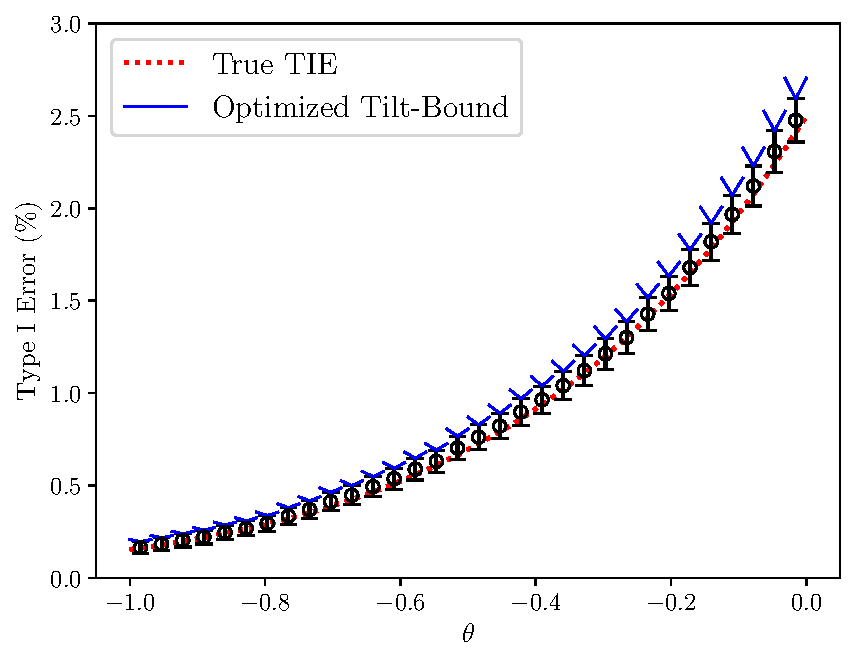
\includegraphics[width=0.95\linewidth]{figs/validation_32.pdf}
\end{figure} 
\end{frame}

\begin{frame}{Use Tilt-Bound on a Grid for the Z-Test}
\begin{figure}
    \centering
    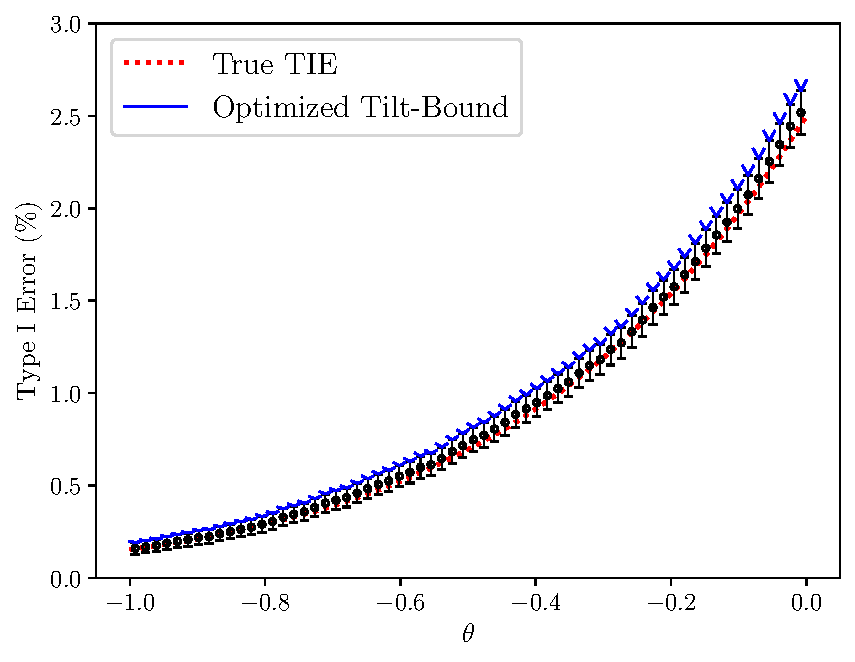
\includegraphics[width=0.95\linewidth]{figs/validation_64.pdf}
\end{figure} 
\end{frame}